% Matteo Kumar
% PPB2 AFM
%Grundlagen

\chapter{Grundlagen}

\section{FRET}

Förster-Resonanzenergietransfer ist ein Prozess des Energietransfers. Dabei gibt es einen Donor und einen Akzeptor. Der Donor gibt dabei über Dipol-Dipol-Wechselwirkung 
Energie an den Akzeptor ab – und das strahlungsfrei.
Damit FRET auftritt müssen bestimmte Voraussetzungen erfüllt sein. Zunächst müssen sich das Emissionsspektrum des Donors und das Absorptionsspektrum des Akzeptors überlappen wie in  
Abbildung \ref{bild:FRETSpektrum} zu sehen.

\begin{figure}[h]
    \centering
    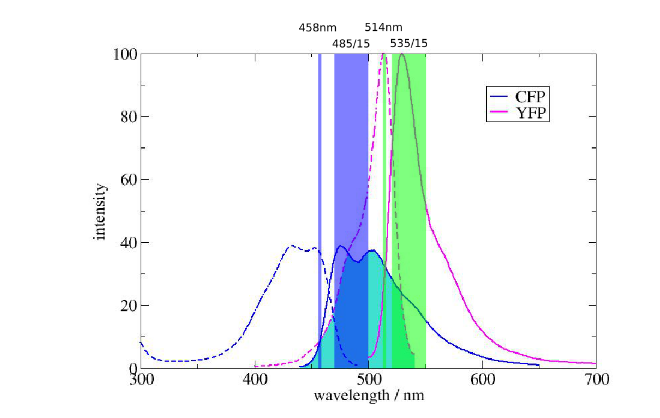
\includegraphics[width = 10cm]{Bilder/Grundlagen/FRETSpektrum.png}
    \caption{Emissionsspektrum/Absorptionsspektrum von CPF/YFP (\cite{FRETSkript})}
    \label{bild:FRETSpektrum}
\end{figure}

Sollte dies der Fall und der Abstand zwischen Akzeptor und Donor klein genug sein, dann tritt FRET auf. \\
Der Abstand muss klein genug sein, da die FRET-Effizienz\\


\begin{equation}
    E = \frac{1}{1+\frac{r^6}{R_0^6}}
\end{equation}

ist. Dabei bezeichnet $R_0$ den Försterradius und $r$ den Abstand der beiden Moleküle. Man sieht seht schön, dass $E = 1/2$ ist für $r = R_0$. Das ist auch die 
Definition des Försterradiuses: Die Hälfte der einfallenden Photonen, die vom Donor absorbiert werden, werden über FRET auf den Akzeptor übertragen.\\
Der Försterradius liegt normalerweise im Nanometerbereich, da die Dipol-Dipol-Wechselwirkung sehr kurzreichweitig ist. Daher kommt auch die sechste Potenz unter dem Bruchstrich.\\
Wichig ist noch, dass ein Teil der Energie als Vibration bei dem emittierenden Molekül bleibt. Daher ist die emittierte Strahlungen energieärmer als die absorbierte Strahlungen. Außerdem 
ist der Prozess stark orientierungsabhängig, da Dipole dies auch sind.


\section{Photobleichung}

Die Photobleichung ist ein Prozess, bei dem die Fluoreszenzeigenschaften einen Fluorophors vollständig verloren gehen. 
Dies geschieht, indem man das Fluorophor mehrfach anregt. Ein Fluorophor hat eine durchschnittliche Anzahl an Anregungs- und Emissionszyklen. 
Bei zu häufiger Anregung wir das Fluorophor inaktiviert, indem es im Molekül zu einer photochemischen 
Reaktion kommt. Dabei kann ein Elektron, was auf eine höhere Schale gehoben wurde, zu irreversibel kovalenten Änderung am 
Fluorophor führen (\cite{Song1995}).

\section{Konfokalmikroskop}

Ein Konfokalmikroskop (siehe Abb. \ref{bild:Konfokalmikroskop}) ist ein Mikroskop, was im Gegensatz zum klassischen Mikroskop nicht die gesamte Probe beleuchtet. 
Stattdessen beleuchtet es Punktweise die Probe mit einem Laserstrahl. Danach detektiert man die zurückfallende Strahlung, 
beispielsweise bei Fluorophoren die Fluoreszenz. Diese wird durch eine Lochblende geführt, sodass bei kleiner 
Blendenöffnung nur Punkte in einer bestimmten Ebene angezeigt werden. Bei größerer Blende ist die Lichtstärke höher, die betrachtete Ebene ist aber auch tiefer. 

\begin{figure}[ht]
    \centering
    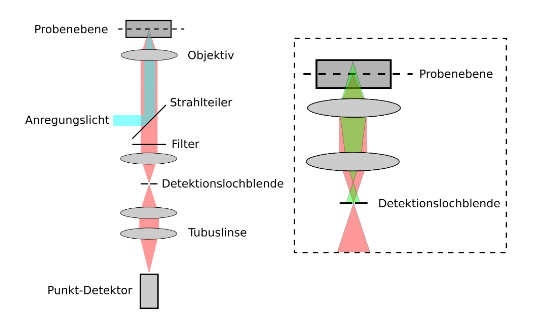
\includegraphics[width = 10cm]{Bilder/Grundlagen/Konfokalmikroskop.png}
    \caption{Skizze eines Konfokalmikroskops und Prinzip der selektiven Detektion (\cite{FRETSkript})}
    \label{bild:Konfokalmikroskop}
\end{figure}

Bei diesem Mikroskop entsteht also zu keinem Zeitpunkt ein vollständiges Bild. Es eignet sich besonders zum untersuchen biologischer Proben. 
Dabei versetzt man diese mit einem fluoreszenten Protein, welches den entsprechden Arealen anhaftet, und mikroskopiert dieses dann. Dadurch kann man 
deutlich kontrastreichere Bilder aufnehmen und beispielsweise Membrane sichtbar machen. 